\documentclass[11pt]{article}
\usepackage[utf8]{inputenc}
\usepackage[T1]{fontenc}
\usepackage[spanish,es-tabla]{babel} % idiomas (uno o varios)

\usepackage[left = 2.25cm, right = 2.25cm, top=1.5cm, bottom = 1.5cm]{geometry}
\usepackage{mathtools} % símbolos extensibles (contiene amsmath)
\usepackage{amssymb} % símbolos matemáticos
\usepackage{mathrsfs} % para usar \mathscr{}
\usepackage{physics} % notación de Dirac
\usepackage{tensor} % índices en cualquier lado

\usepackage{booktabs} % tablas
\usepackage[bookmarks = true, colorlinks=true, linkcolor = black, citecolor = black, menucolor = black, urlcolor = black]{hyperref} % para referencias cruzadas
\usepackage[table]{xcolor} % colores (incluye colortbl la cargarlo con table)
\usepackage{tcolorbox} % cajas de colores con titulo

\usepackage{float} % para figuras (las fija, [H], ...)
\usepackage{graphicx} % para figuras
\usepackage{caption} % pie de foto
\usepackage{subcaption} % pie de ''subfoto''


\selectlanguage{spanish}
\renewcommand{\theenumi}{\roman{enumi}}
\renewcommand{\thefigure}{\Roman{figure}} 
\newcommand\diagram[2]{\schema{\schemabox{#1}}{\schemabox{#2}}}

\begin{document}

\subsubsection*{Ejercicio 1}

\begin{itemize}
    \item Distancias:
    \begin{table}[H]
    \centering
    \begin{tabular}{cccccc}
    \hline
    $X_1$ & $X_2$ & $X_3$ & $X_4$ & $X_5$ & $X_6$ \\ \hline
    $\sqrt{13} \approx 3.605551$ & $\sqrt{18} \approx 4.242641$ & $\sqrt{10} \approx 3.162278$ & $3$ & $\sqrt{6} \approx 2.449490$ & $\sqrt{5} \approx 2.236068$ \\
    \end{tabular}
    \end{table}
    \item \textbf{Para $K = 1$:} $Y = 0$ (muestra $6$).
    \item \textbf{Para $K = 3$:} $Y = 1$ (muestras $6, 5, 4$).
\end{itemize}

\subsubsection*{Ejercicio 2}

\begin{itemize}
    \item \textbf{Menor error de validación cruzada, su desviación estándar y valor de $K$:} $\Delta = 0.202283$, $\sigma = 0.022126$, $K = 32$.
    \item \textbf{Con regla de una desviación estándar:} $\Delta = 0.219034$, $\sigma = 0.021042$, $K = 47$.
    \begin{figure}[H]
    \centering
    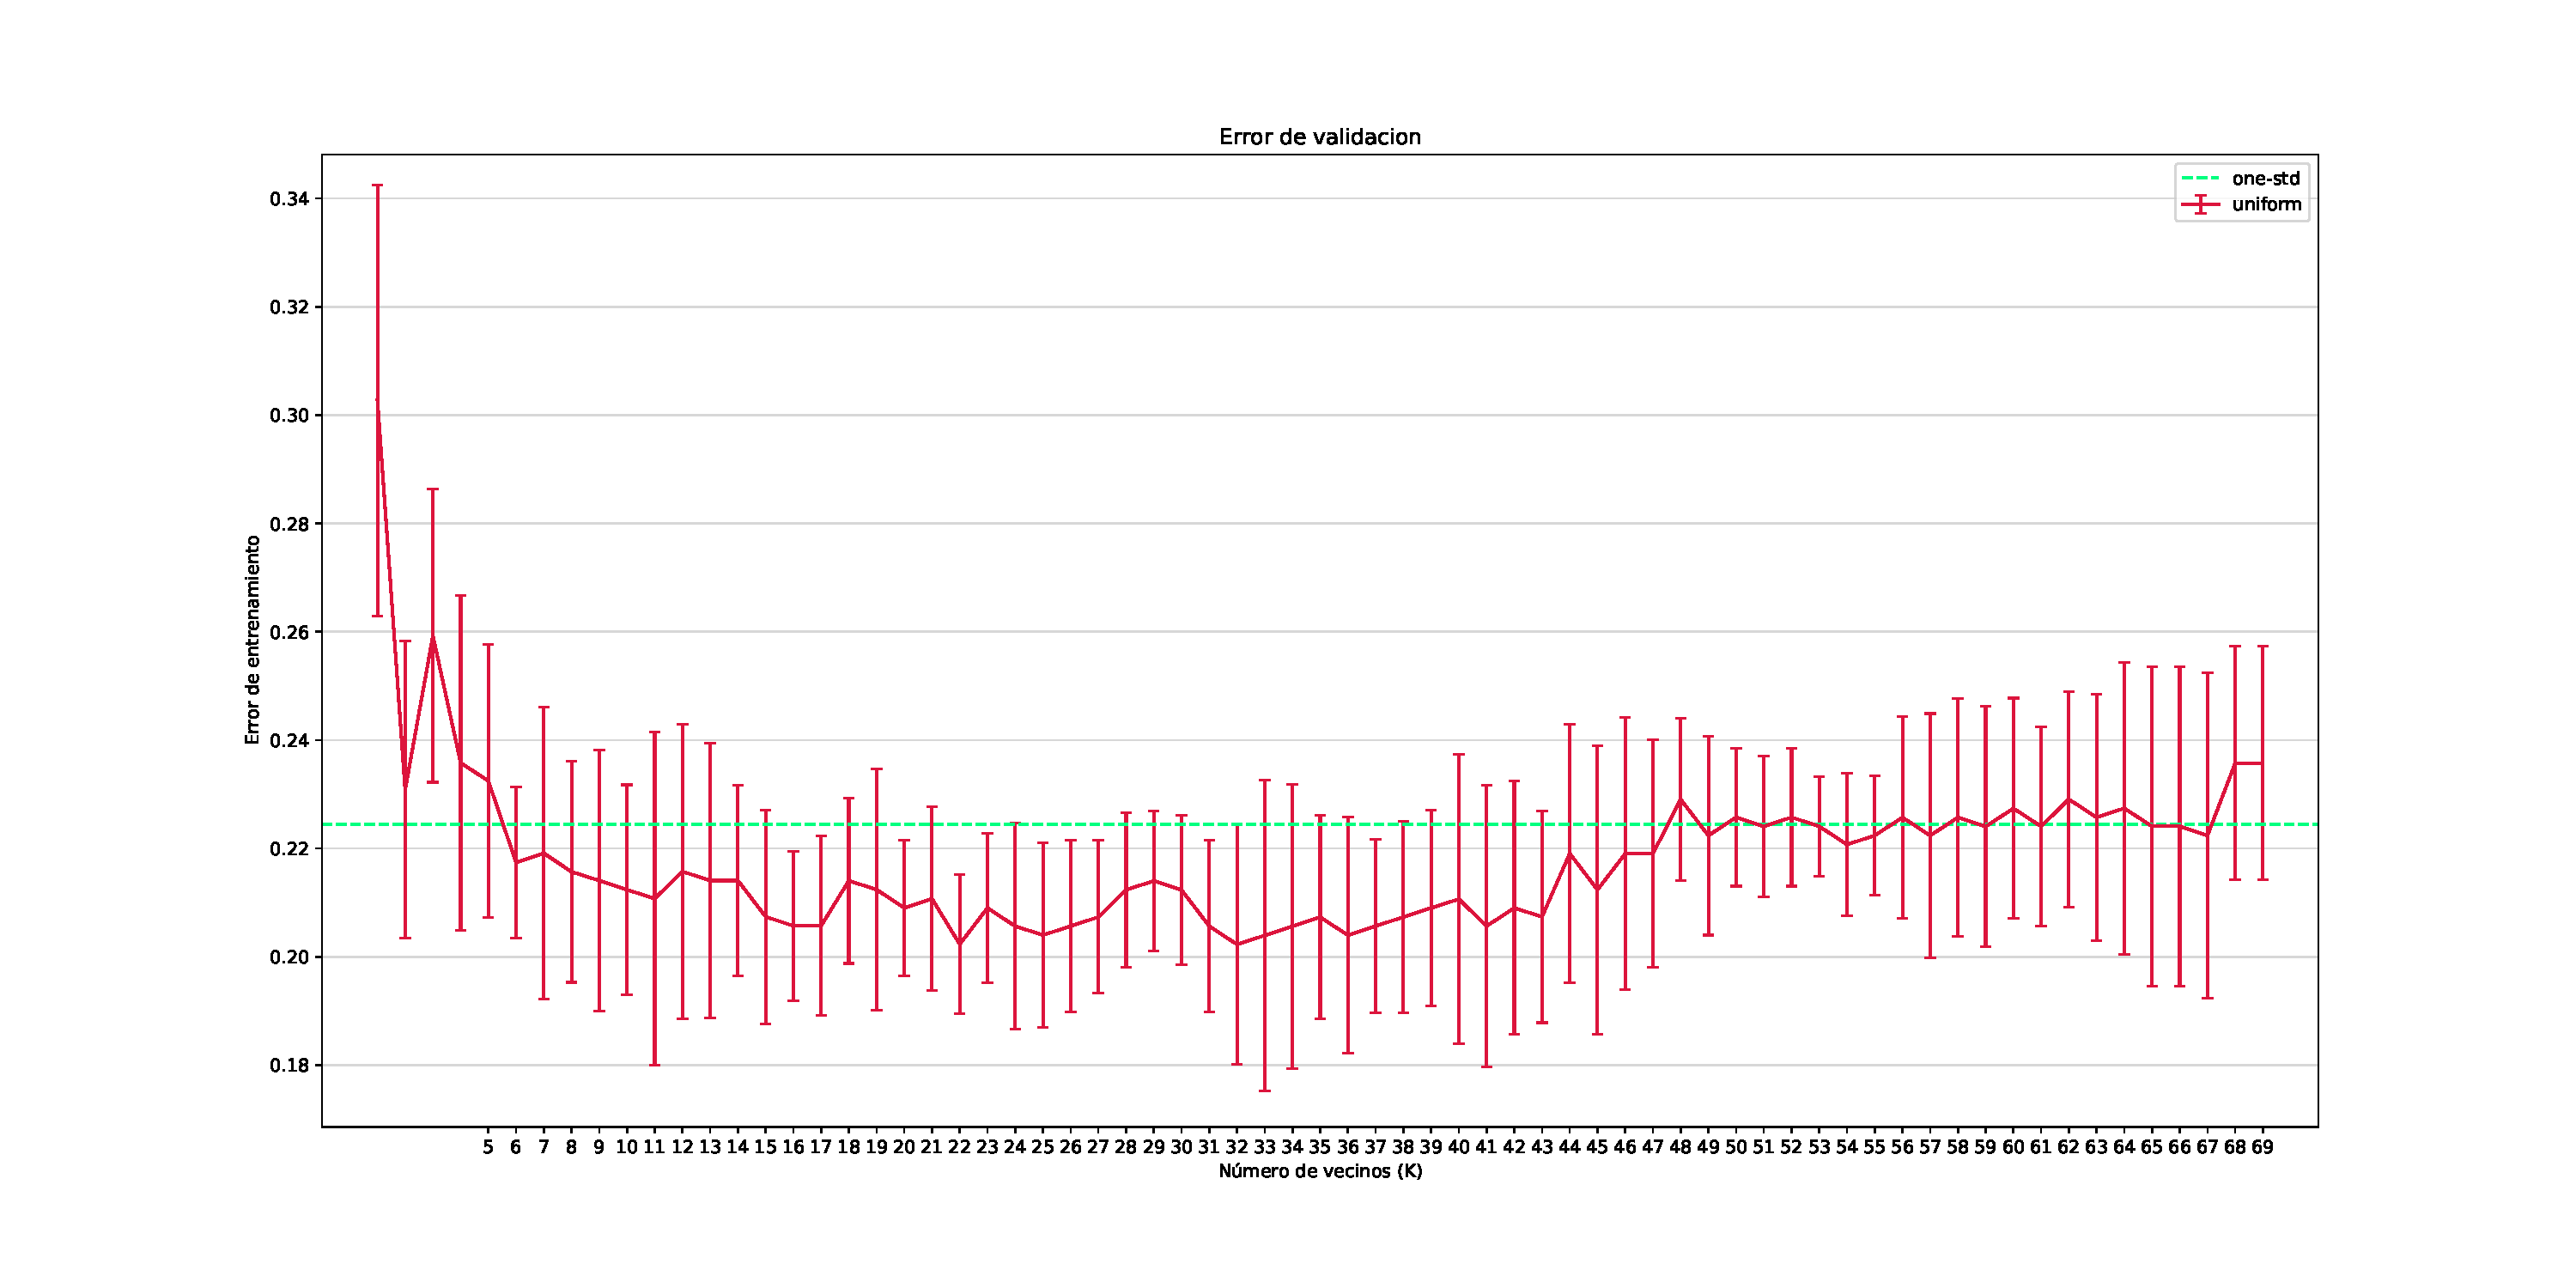
\includegraphics[width=0.9\textwidth]{fotos/ej2_1.pdf}
    \end{figure}
    \item \textbf{Error de test para el K de validación cruzada:} $\Delta = 0.213333$, $K = 32$.
    \begin{figure}[H]
    \centering
    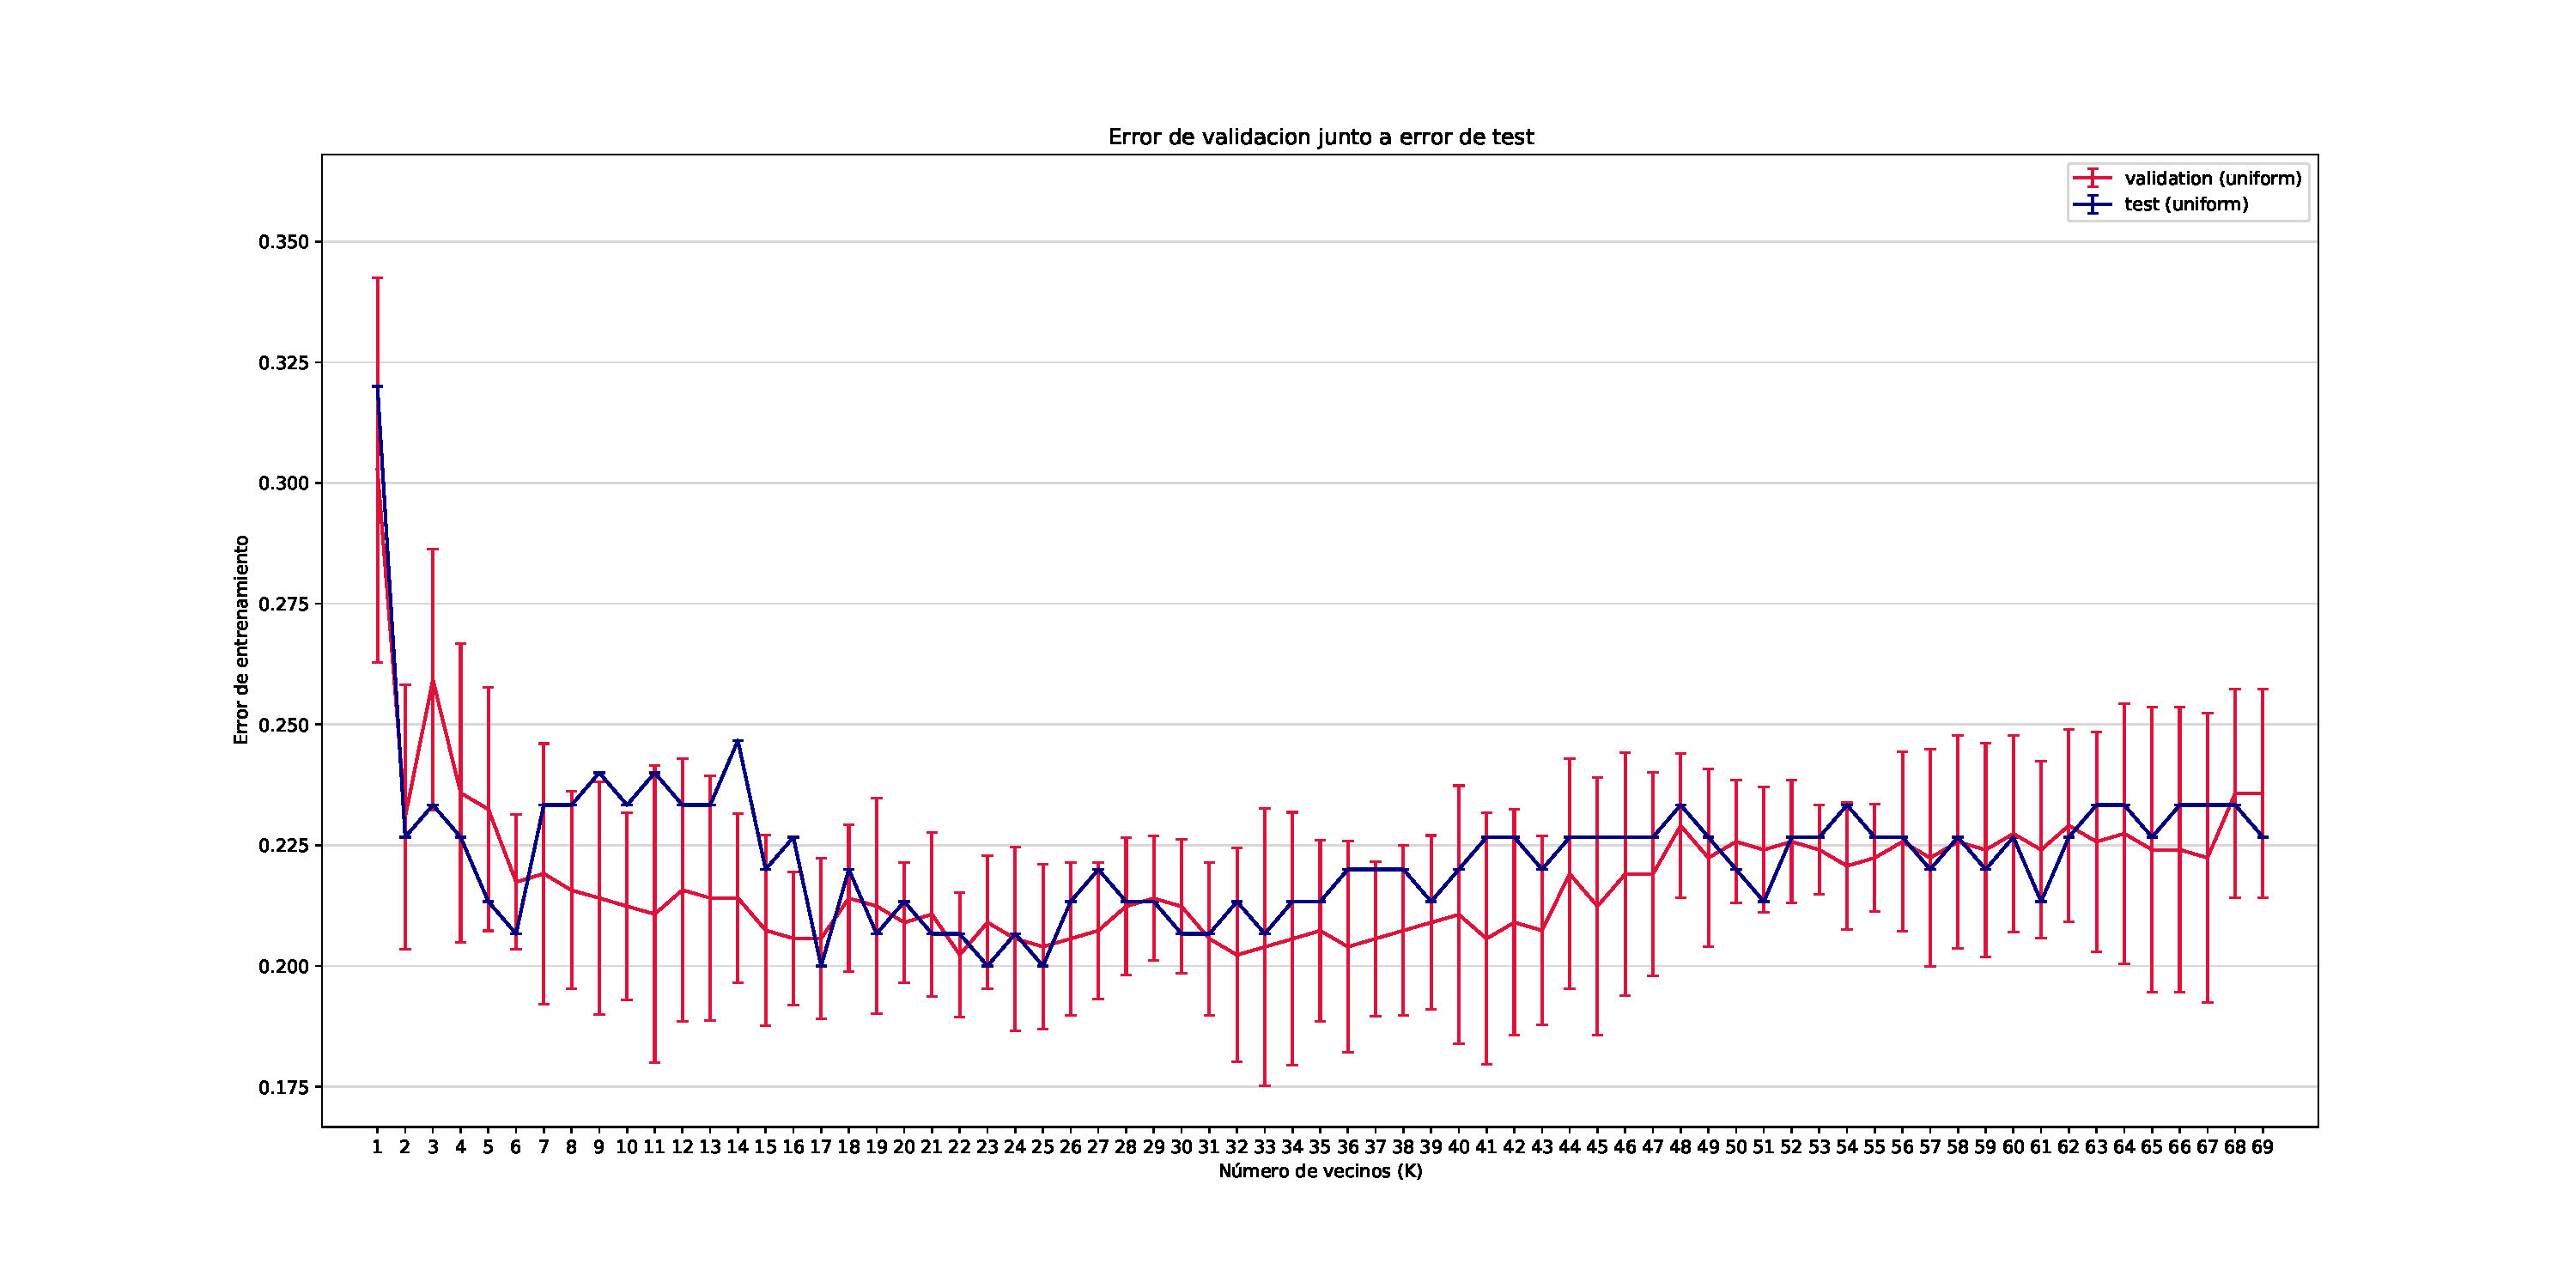
\includegraphics[width=0.9\textwidth]{fotos/ej2_2.pdf}
    \end{figure}
\end{itemize}


\subsubsection*{Ejercicio 3}

\begin{itemize}
    \item \textbf{Menor error de validación cruzada, su desviación estándar y valor de K:} $\text{MSE} = 6.115019$, $\sigma = 0.577814$, $K = 2$.
    \item \textbf{Con regla de una desviación estándar:} $\text{MSE} = 6.115019$, $\sigma = 0.577814$, $K = 2$.
    \begin{figure}[H]
    \centering
    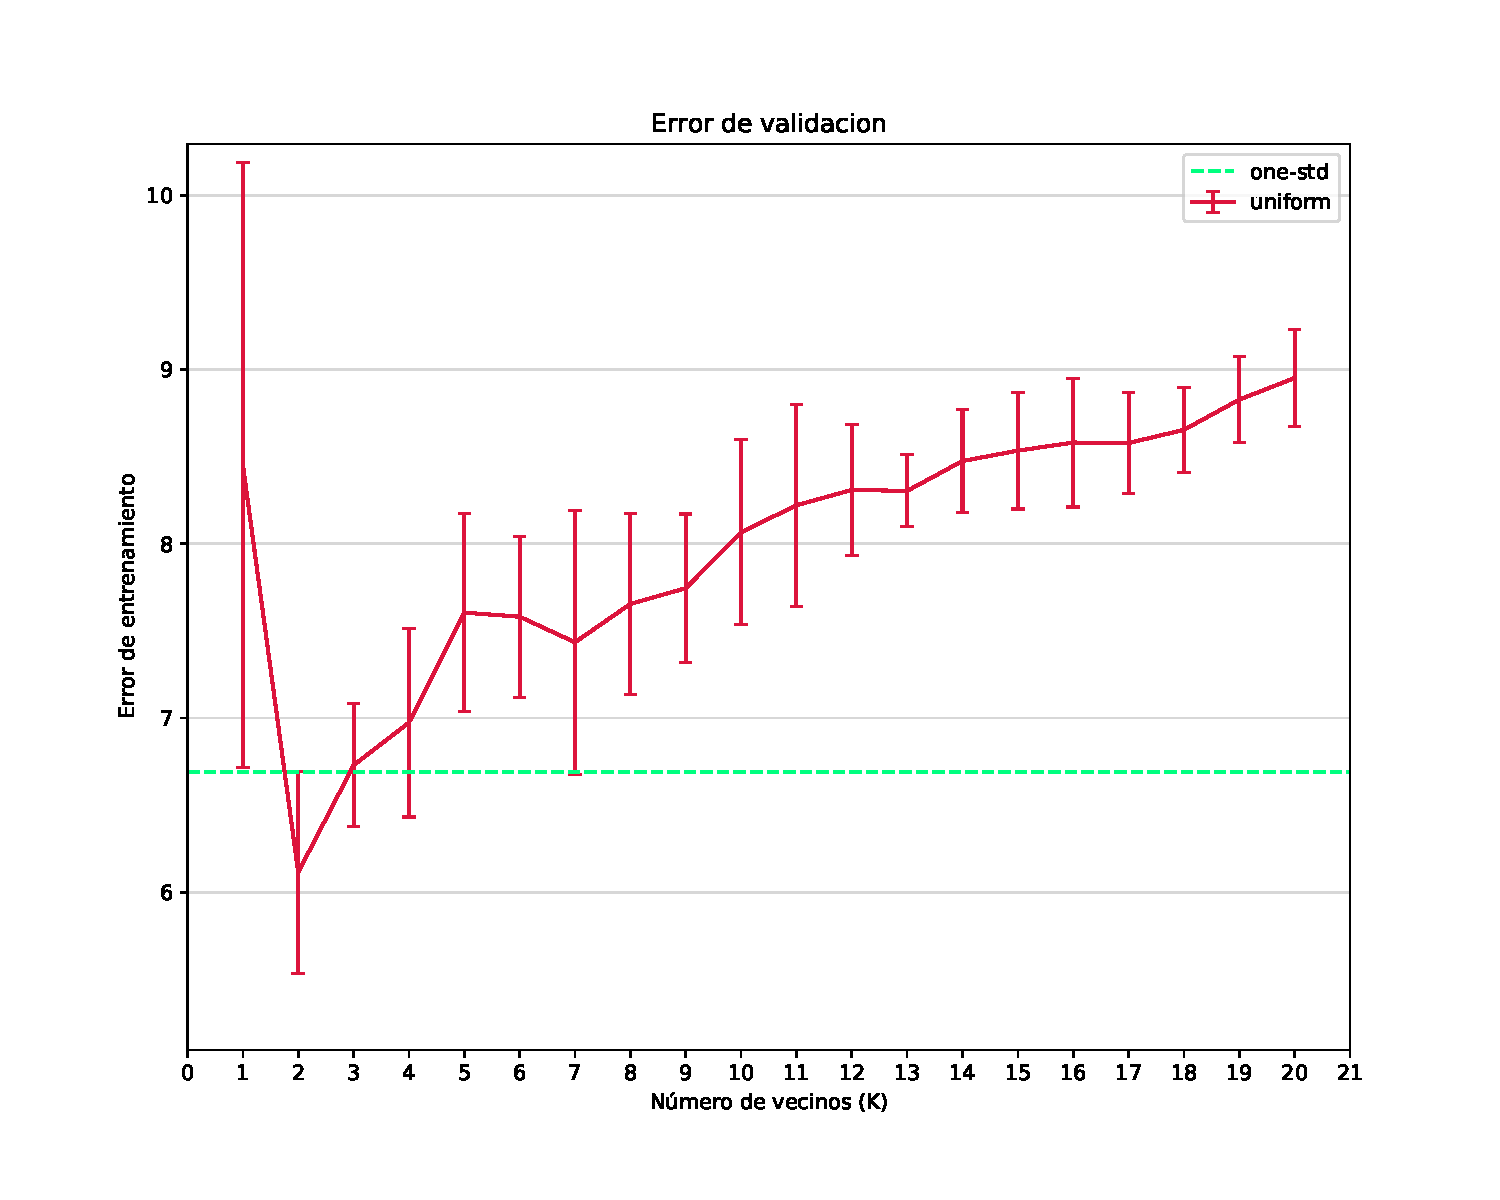
\includegraphics[width=0.75\textwidth]{fotos/ej3_1.pdf}
    \end{figure}
    \item \textbf{Error de test para el K de validación cruzada:} $\text{MSE} = 12.588656$, $K = 2$.
    \begin{figure}[H]
    \centering
    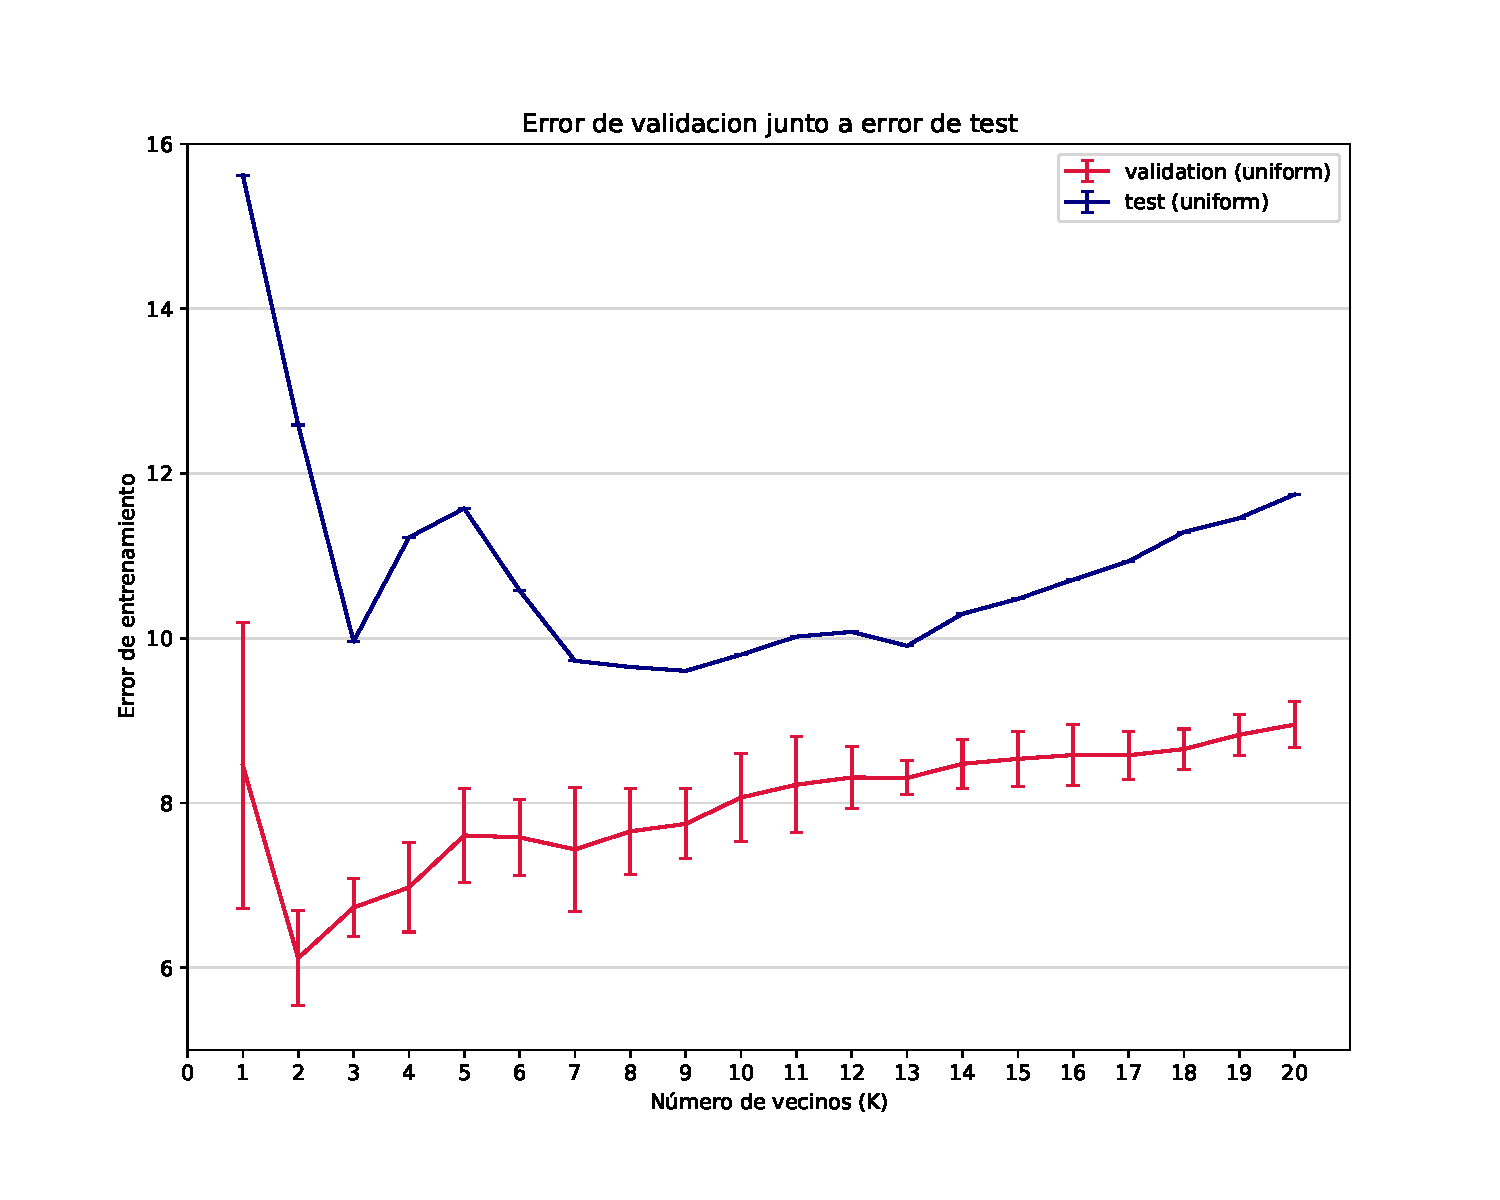
\includegraphics[width=0.75\textwidth]{fotos/ej3_2.pdf}
    \end{figure}
\end{itemize}


\end{document}
